\textbf{Re-visiting the Computation Challenge}~~
\begin{figure}
    \subfigure[Iterative Evaluation]{\label{fig:itERR}
      \begin{minipage}[l]{0.46\columnwidth}
        \centering
        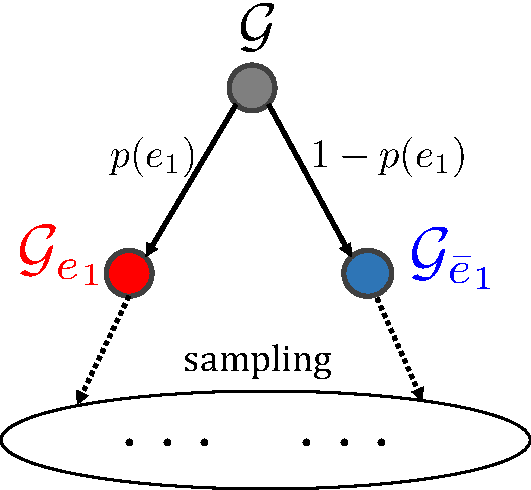
\includegraphics[height=2.7cm]{figure/iterativeERR.pdf}
      \end{minipage}
      }
    \subfigure[Memorized Evaluation]{\label{fig:groupERR}
      \begin{minipage}[l]{0.46\columnwidth}
        \centering
        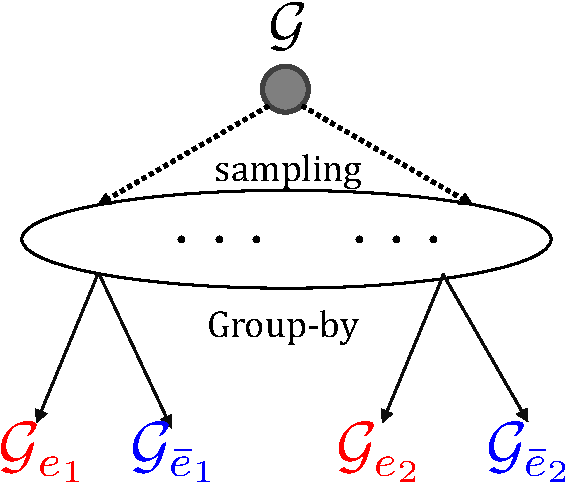
\includegraphics[height=2.7cm]{figure/groupERR.pdf}
      \end{minipage}
      }
    \vspace{-10pt}
    \caption{Sampling-based reliability detection}
    \vspace{-5pt}
    \label{fig:computationERR}
\end{figure} 
% At the first glance, the evaluation of $\mathcal{E}RR(e)$ 
The remaining question is to calculate
As shown in Equation~\ref{eq:err},  
the evaluation of $\mathcal{E}RR(e)$ involves a fundamental problem concerning uncertain graphs, which we call 
the Two-Terminal Reliability detection (TTR) problem. 
Since this problem is \#P-complete, we focus on efficiently and accurately approximate TTR.
The Monte-Carlo sampling method can be used to estimate the underlying reliability of an uncertain graph. 
Namely, we create a subset of possible worlds of the given uncertain graph with the use of edge sampling probabilities. 
Then, we take the average of the number of connected node pairs in the sampled worlds as an approximation. 
 
It is not trivial to evaluate $\mathcal{E}RR$ over all the edges. 
One option is to iteratively invoke the sampling-based reliability computation over all the edges, 
as illustrated in Figure~\ref{fig:itERR}. 
It is straightforward to compute the connected components of a graph in linear time (regarding the numbers of the nodes and edges of the graph) using either breadth-first search or depth-first search.
For each edge, we need to perform the connected component detection for $N$ sampled graphs.
Thus, the overall time complexity is typically in the order of $\mathcal{O}( N |E|^{2})$.
Apparently, the iterative evaluation is inefficient when the uncertain input graph is massive.

Here, we present an efficient method with the time complexity in the order of $\mathcal{O}(N |E|)$.
As illustrated in Figure~\ref{fig:groupERR}, it memories the connected components detection result of samples. 
For evaluating the reliability relevance of one edge $e$, we group the sampled possible worlds according to the edge existence, 
then get the average value of $cc$ over each group as accurate approximation of $cc(\mathcal{G}_{e})$ and $cc(\mathcal{G}_{\bar{e}})$. 
Instead of sampling and evaluation from the scratch, we utilized the memorized results. 
The running time analysis roughly follows the analysis of the single-edge case.  
By this way, we bring the evaluation of edge reliability relevance to the realm.